\documentclass{beamer}
\usetheme{Madrid}
%\usecolortheme{orchid}
\usecolortheme[rgb={0,0.4,0}]{structure}

%\usepackage[utf8]{inputenc}
\usepackage{pifont,eqnarray,amsmath,minted,bm}
\usepackage[ruled,vlined,linesnumbered]{algorithm2e}


\title[CNN, ResNet]{Convolutional and residual neural networks}
\subtitle{An overview}

\author{Simon Jacquet}
\institute[Unamur]{Faculty of Computer Science\\Unamur}

\date{March 1st 2022}

\logo{
\includegraphics[height=1cm]{images/logo unamur.png}}

%\newcommand{\matr}[1]{\mathbf{#1}} % undergraduate algebra version
%\newcommand{\matr}[1]{#1}          % pure math version
\newcommand{\matr}[1]{\bm{#1}}     % ISO complying version


\begin{document}

\maketitle

\begin{frame}{Content}

\vfill
\begin{itemize}
    \item Neural networks
    \begin{itemize}
        \item Structure
        \item Activation functions
        \item Loss function
    \end{itemize}
    \vfill
    \item Convolutional neural network (CNN or ConvNet)
    \begin{itemize}
        \item Convolution
        \item Pooling
        \item Fully connected layers
        \item Dropout
    \end{itemize}
    \vfill
    \item Residual neural network (ResNet)
    \begin{itemize}
        \item ResNet 18
        \item Basic block
        \item Batch normalization
    \end{itemize}
\end{itemize}
\vfill
    
\end{frame}

\begin{frame}{Neural networks}

\begin{figure}
    \centering
    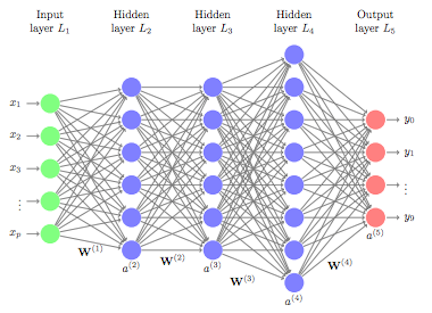
\includegraphics[scale=0.4]{images/neuralnetwork.png}
    \label{fig:nn}
\end{figure}
    
\begin{itemize}
    \item Where $a^{(l)} = \sigma^{(l)}(\matr{W}^{(l-1)} a^{(l-1)} + b^{(l-1)})$, with:
    \begin{itemize}
        \item $l$, the layer number
        \item $\sigma^(l)$, the activation function at layer $l$
        \item $\matr{W}^(l)$, the weights between layers $l$ and $l+1$
        \item $b^{(l)}$, the bias
    \end{itemize}
\end{itemize}
    
\end{frame}

\begin{frame}{Neural networks: activation function}

\begin{figure}
    \centering
    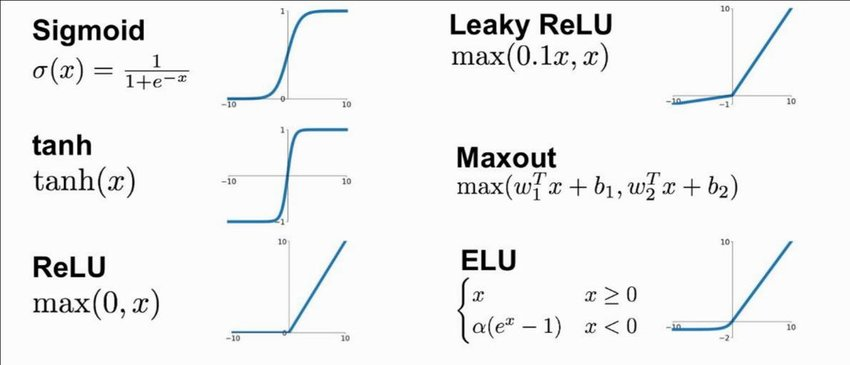
\includegraphics[scale=0.4]{images/Activation functions.png}
    \label{fig:my_label}
\end{figure}

\begin{itemize}
    \item There are many activation functions
    \item The two most common are the sigmoid and ReLU (Rectified Linear Unit)
    \item In deep learning, the sigmoid is typically used in the last layer and ReLU everywhere else
\end{itemize}
    
\end{frame}

\begin{frame}{Neural networks: loss function}
    

\begin{figure}
    \centering
    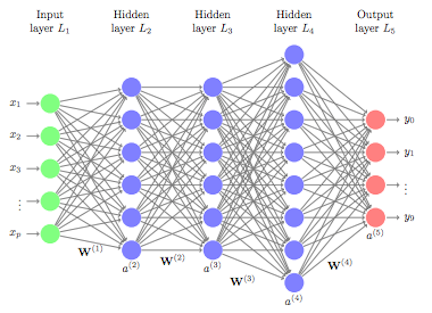
\includegraphics[scale=0.4]{images/neuralnetwork.png}
    \label{fig:nn}
\end{figure}
    
\begin{itemize}
    \item Loss function: $L_{CE}(x) = - \displaystyle\sum_{i=1} ^{m} t_i \log(y_i)$ with 
    \begin{itemize}
        \item $y$ the predicted output of $x$,
        \item $t$ the true output of $x$
        \item $CE$ for cross entropy
    \end{itemize}
\end{itemize}
    
\end{frame}


\begin{frame}{Convolutional neural networks (CNNs or ConvNets)}

\begin{figure}
    \centering
    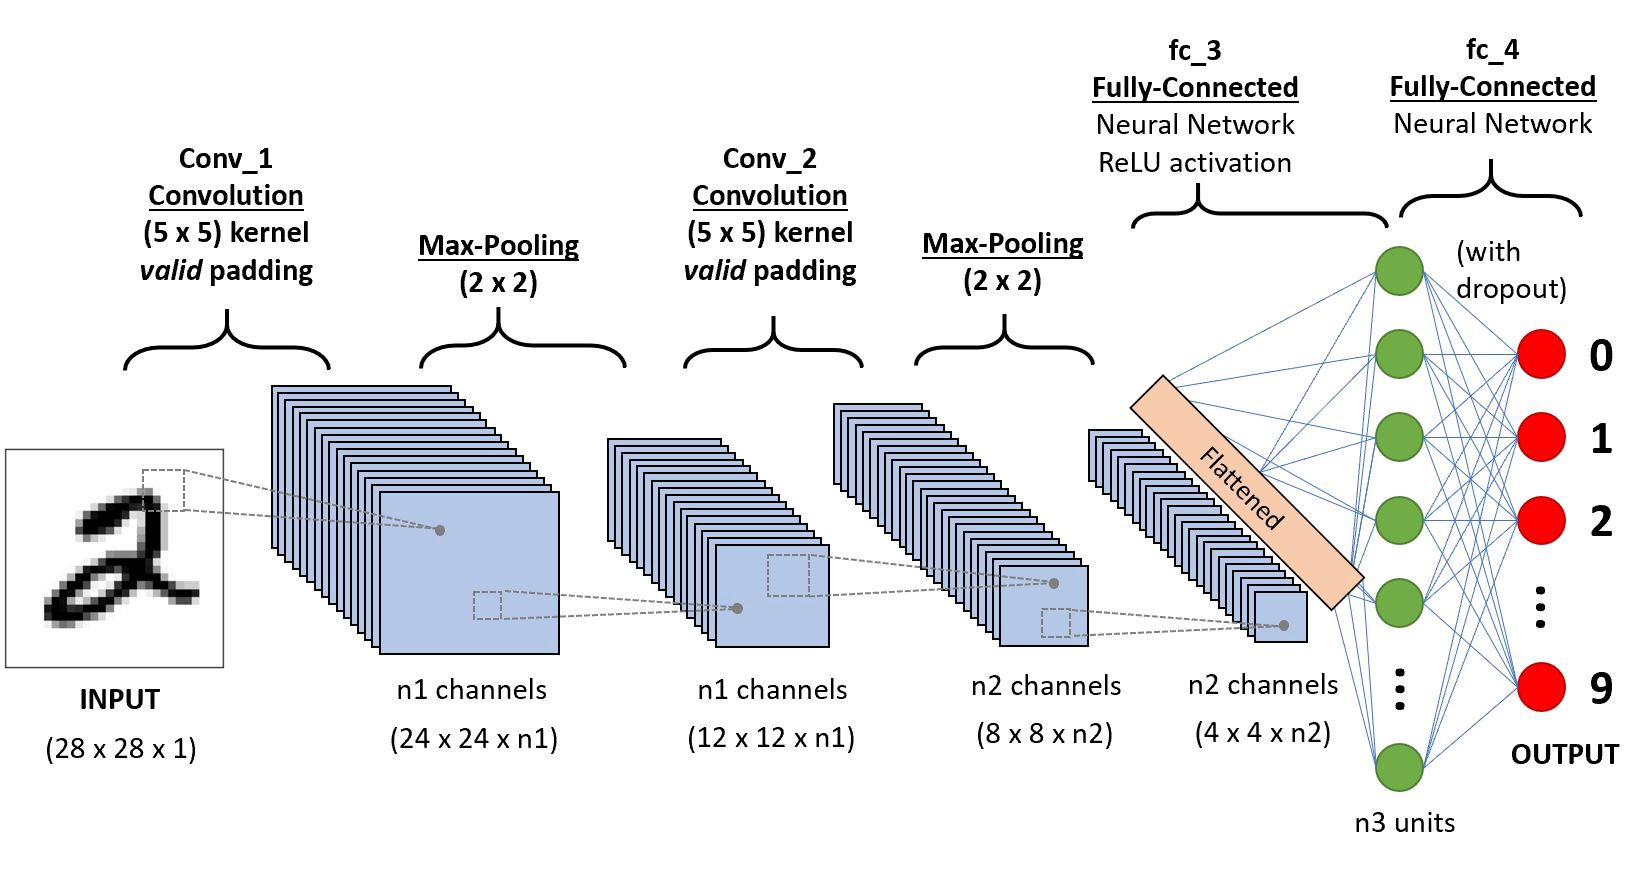
\includegraphics[scale=0.15]{images/CNN for image.jpeg}
\end{figure}
\begin{itemize}
    \item New concepts:
    \begin{itemize}
        \item Convolution
        \item Pooling
        \item Fully connected layers
        \item Dropout (for better training)
    \end{itemize}
\end{itemize}
    
\end{frame}

\begin{frame}{ConvNets: Convolution}

\begin{figure}
    \centering
    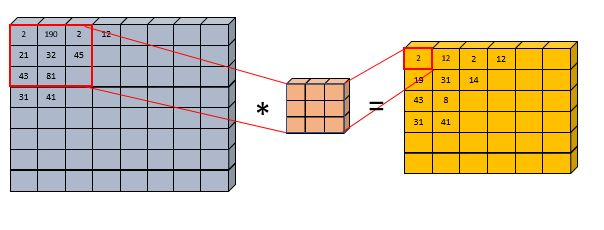
\includegraphics[scale=0.6]{images/convolutionkernel.JPG}
\end{figure}
\vspace*{-1cm}
\begin{itemize}
\item $x * k = y$, with 
\begin{itemize}
    \item $*$, the convolution symbol,
    \item $x$, the input image,
    \item $k$, the kernel,
    \item $y$ the output image
\end{itemize}
\vfill
\item $y[i,j] = \sum_{i'=0,j'=0} ^{i'<k_1,j'<k_2} x[i+i',j+j'] \ k[i',j']$
\vfill
\item Padding:
\begin{itemize}
    \item \textsc{VALID}: $y$ keeps the size of $x$, with added zeros
    \item \textsc{SAME}: $y$ has a smaller size than $x$
\end{itemize}
\end{itemize}
    
\end{frame}

\begin{frame}{ConvNets: Pooling}

\begin{figure}
    \centering
    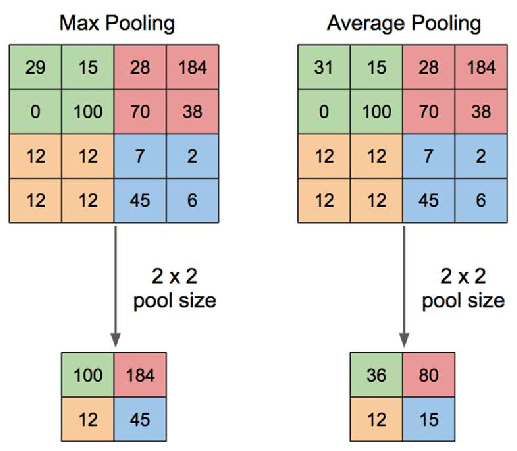
\includegraphics[scale=0.3]{images/Pooling methods.png}
\end{figure}

\begin{itemize}
    \item Reduce the dimensions of the feature maps \footnote{\label{ref1}https://www.geeksforgeeks.org/cnn-introduction-to-pooling-layer/}
    \item Summarises the features present in a region of the feature map generated by a convolution layer \footnotemark[1]
\end{itemize}
\end{frame}

\begin{frame}{ConvNets: Dropout}
\begin{figure}
    \centering
    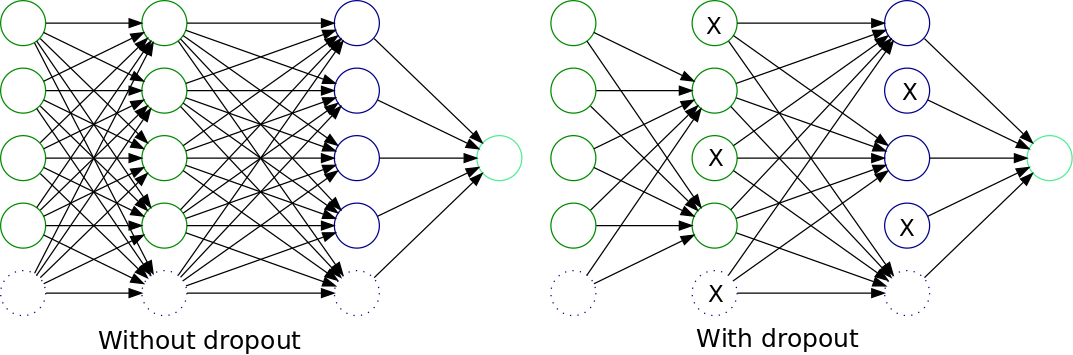
\includegraphics[scale=0.3]{images/Dropout.png}
\end{figure}

\begin{itemize}
    \item Parameter: $d$, the drop rate
    \item $\hat{a}_i^{(l)} =
    \begin{cases}
      0, & \text{with probability }d \\
      a_i^{(l)}, & \text{otherwise}
    \end{cases}$
    \item Happens only during training
    \item Reduce overfitting by preventing complex co-adaptations on training data.
\end{itemize}
    
\end{frame}

\begin{frame}{ConvNets for text: embedding}
\begin{figure}
    \centering
    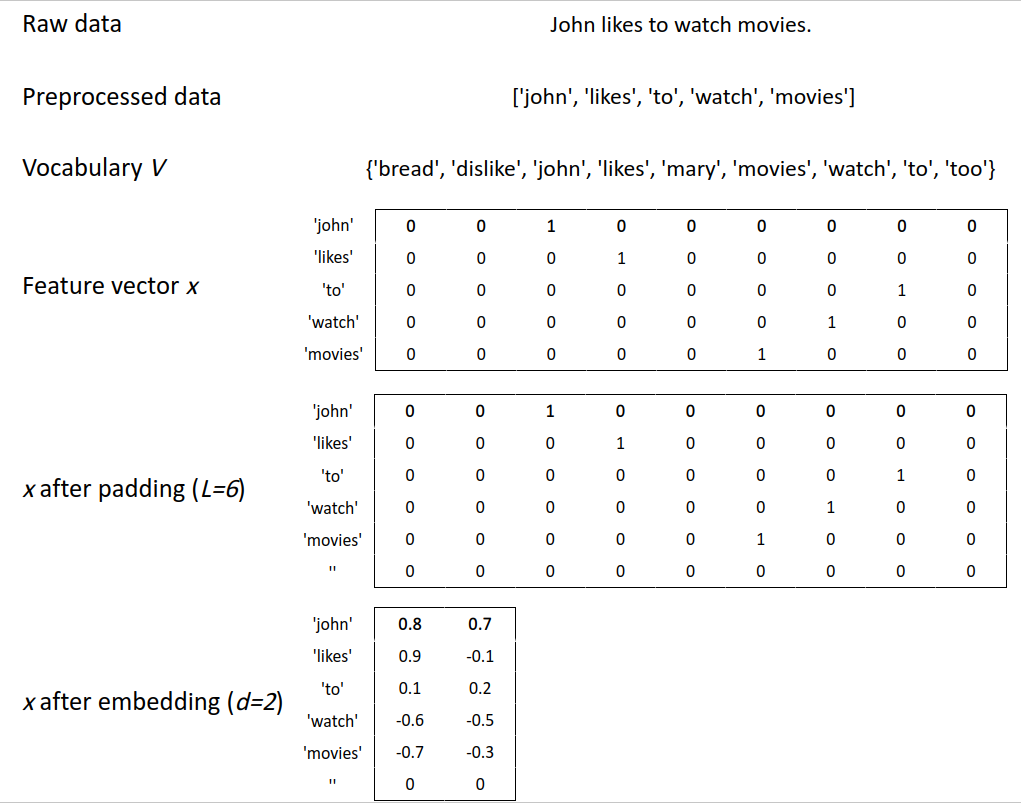
\includegraphics[scale=0.28]{images/Embedding.png}
\end{figure}    
\end{frame}

\begin{frame}{ConvNets for text: example of architecture}
\begin{figure}
    \centering
    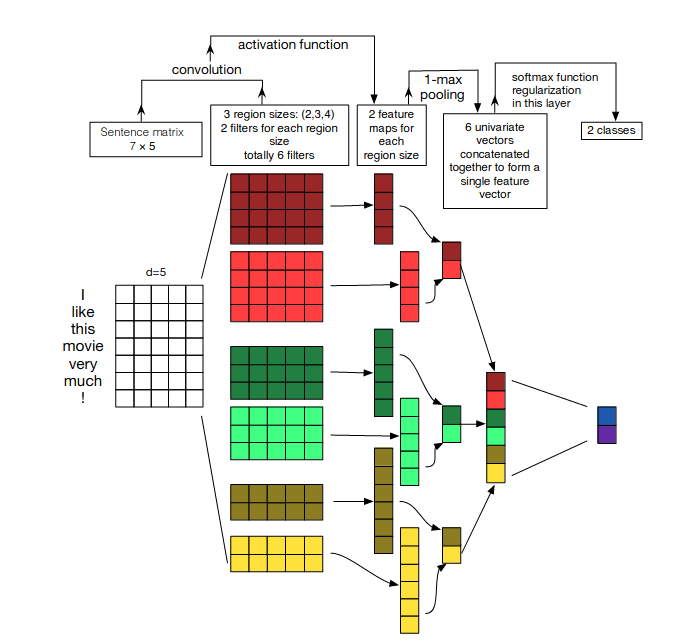
\includegraphics[scale=0.35]{images/cnnstruct.png}
\end{figure}    
\end{frame}

\begin{frame}{ResNet 18}

\begin{figure}
    \centering
    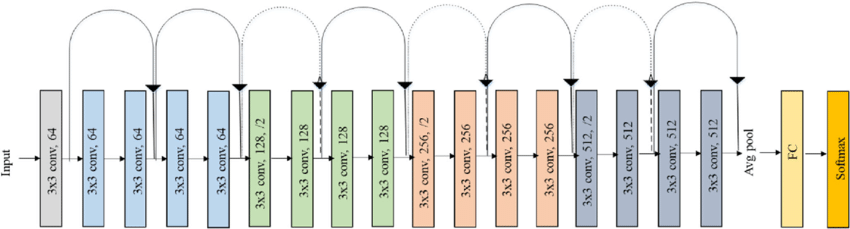
\includegraphics[scale=0.4]{images/resnet18image.png}
\end{figure}


\noindent\begin{minipage}{0.6\textwidth}% adapt widths of minipages to your needs
\begin{itemize}
    \item Utilize skip connections
    \item Typically, two or three layer skips
    \item Uses batch normalization
    \begin{itemize}
        \item[\ding{43}] method used to make artificial neural networks faster and more stable
    \end{itemize}
\end{itemize}

\end{minipage}%
\hfill%
\begin{minipage}{0.3\textwidth}\raggedleft
\begin{figure}
    \centering
    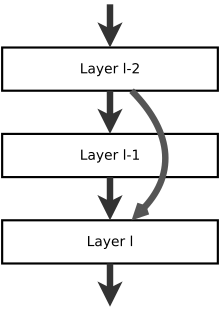
\includegraphics[scale=0.3]{ResNet_canonicalform.png}
\end{figure}
\end{minipage}


    
\end{frame}

\begin{frame}{ResNet 18: Details}
\begin{figure}
    \centering
    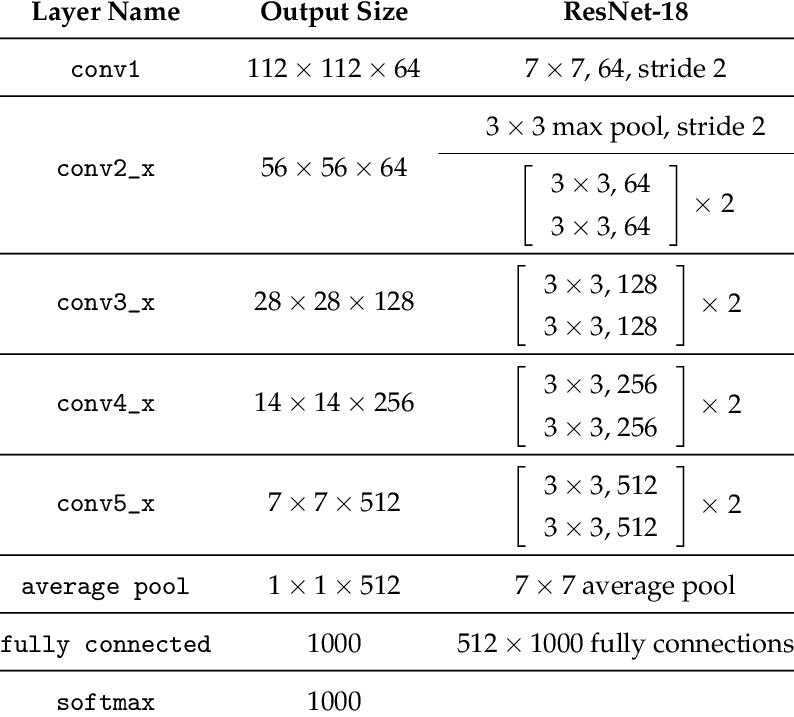
\includegraphics[scale=0.3]{images/resnet18table.png}
\end{figure}    
\end{frame}

\begin{frame}{ResNet: Basic block}

\begin{figure}
    \centering
    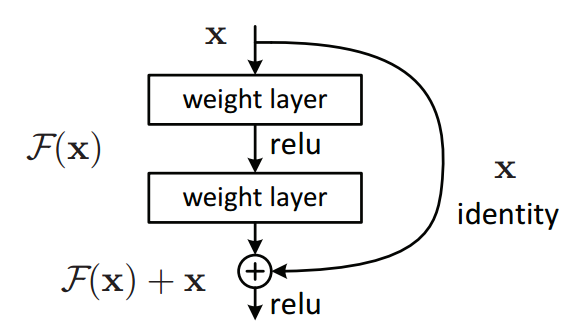
\includegraphics[scale=0.3]{images/basicblock.png}
\end{figure}

\begin{itemize}
    \item Reasons:
    \begin{itemize}
        \item Avoid the problem of vanishing gradients
        \begin{itemize}
            \item[\ding{43}] Gradients are proportional to the partial derivative wrt. the current weight and can quickly vanish
            \item[\ding{43}] Residual neural networks provide 'highways' for the gradient
        \end{itemize}
        \item Address the Degradation problem
        \begin{itemize}
            \item[\ding{43}] with increasing network depth, accuracy gets saturated and then degrades quickly
        \end{itemize}
    \end{itemize}
\end{itemize}
    
\end{frame}

\begin{frame}{ResNet: Batch normalization}
    
\begin{figure}
    \centering
    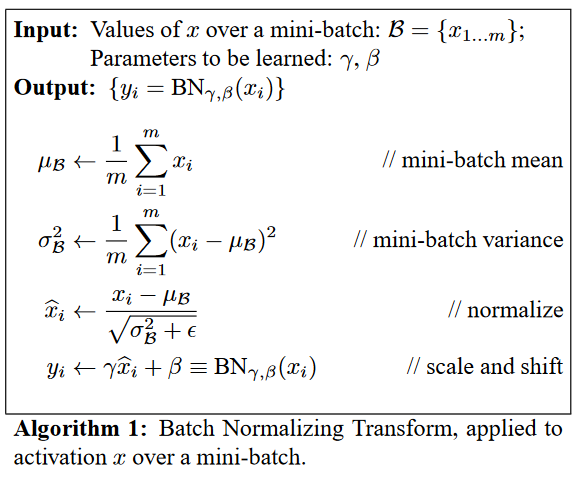
\includegraphics[scale=0.47]{images/BatchNormalization1.png}
\end{figure}    
    
\begin{itemize}
    \item Method: normalization of the layers' inputs by re-centering and re-scaling
    \item Goal: make artificial neural networks faster and more stable
\end{itemize}    
\end{frame}

\end{document}
